\documentclass{sig-semester}

\pdfpageheight=11in
\pdfpagewidth=8.5in

\usepackage{latexsym}
\usepackage{amsmath}
\usepackage{amssymb}
\usepackage{color}
\usepackage{enumerate}
\usepackage{graphicx}
\usepackage{amssymb}
\usepackage{epstopdf}
\usepackage{xspace}

% These are from candidacy edic.tex
\graphicspath{{./graphics/}}
\DeclareGraphicsExtensions{.pdf,.jpeg,.png}

% Legacy from Christoph's paper:
% \DeclareGraphicsRule{.tif}{png}{.png}{`convert #1 `dirname #1`/`basename #1 .tif`.png}

% When converting eps to pdf, suffix is added to filename. 
% Recommended not to be empty string by http://www.tex.ac.uk/tex-archive/macros/latex/contrib/oberdiek/epstopdf.pdf : page 4, suffix paragraph.
\epstopdfsetup{suffix=-generated}

\newtheorem{theorem}{Theorem}[section]
\newtheorem{proposition}[theorem]{Proposition}
\newtheorem{example}[theorem]{Example}
\newtheorem{remark}[theorem]{Remark}
\newtheorem{todo}[theorem]{ToDo}
\newtheorem{algorithm}[theorem]{Algorithm}
\newtheorem{metatheorem}{Metatheorem}[section]
\newtheorem{definition}[theorem]{Definition}
\newtheorem{property}[theorem]{Property}
\newtheorem{corollary}[theorem]{Corollary}
% \newtheorem{lemma}[theorem]{Lemma}
\newtheorem{conjecture}[theorem]{Conjecture}
\newtheorem{proviso}[theorem]{Proviso}


\title{How to preserve order in distributed computation}


%\numberofauthors{1}
\author{\alignauthor Aleksandar Vitorovic \\[1ex]
\affaddr{Dept.\ of Computer Science} \\
\affaddr{EPFL} \\
\affaddr{aleksandar.vitorovic@epfl.ch}
}

\def\SQL{SQL\xspace}
\def\OLAP{OLAP\xspace}
\def\OLTP{OLTP\xspace}
\def\M3{M3\xspace}
\def\EXORD{actual OLAP update execution order\xspace}

\hyphenation{cau-sality lo-gically}

\begin{document}
\maketitle

\abstract{The goal of this survey is to simplify our initial monolithic design and separate functionalities into layers. The system design should become much easier to comprehend, and it will require significantly less space to explain.\\
}

\keywords{Cumulus layering, Group and Virtual Synchronization, Causality}

\section{Introduction}
\vspace{2mm}
This paper presents issues related to the connection between Cumulus and Distributed Systems. First, terminology used in distributed systems which is related to Cumulus is presented. Second, our algorithms are compared to similar ones known to the community. Then, an exhaustive survey of the group communication systems is performed. Finally, a layered structure of Cumulus is shown, along with the directions for future work.

\section{Terminology}
\vspace{2mm}
\textbf{Logical time.} The Lamport clock mechanism assumes using a logical counter on a process level~\cite{Lamport78}. The counter is incremented on each send event and sent along with a message as msg-counter. On receive, the maximum of a counter and a msg-counter is set as a new counter. The Welch clock~\cite{Welch87} is designed to postpone events arriving from very fast process. The Welch clock assumes no clock advancement on receive event. Each process maintains receive buffer, and event from there are executed when they become equal to a logical clock of a process. 

However, these clocks do not guarantee causality for events on different processes where one counter is smaller than another. Vector clock~\cite{Fidge88, Lamport78} assumes each process maintains its logical clocks from all the processes.

\textbf{Happened-before relation.} The relation is denoted with -> sign, and the following text is copied from~\cite{Lamport78}:
\begin{enumerate}[(1)]
 \item If a and b are events are in the same process, and a comes before b, then a -> b.
 \item If a is the sending of a message by one process and b is the receipt of the same message by another process, then a -> b.
 \item If a -> b and b -> c then a -> c. Two distinct events a and b are said to be concurrent if neither a -> b nor b -> a.
\end{enumerate}

\textbf{Causality: logical preceding/succeeding.} The Logical preceding relation (again, we will use -> sign) is a relation among trigger instantiations in the following way. If a and b are maps in the same statement and a is on lhs in trigger instantiation TSA and b is on lhs in trigger instantiation TSB, then TSB->TSA or TSA->TSB. For any two trigger instantiations, TSA and TSB, if TSA->TSB, then TSA logically precedes TSB and TSB logically succeeds TSA, and they are causally ordered.

Writes do not have to be ordered mutually, because the effect of a write is visible only to read operation. Thus, writes need to be ordered only with all the relevant reads.

\textbf{Causal shuffle.} If by combining all the causal relations in the system no cycles are formed, a causal shuffle is obtained. As a special case of avoiding cycles in a causal shuffle, it is not allowed for multiple maps within the same pair of trigger instantiation to adopt the opposite logical order. Within a single causal shuffle, different nodes may observe different order of trigger instantiations only if there is no logically preceding/succeeding relations among them. The causal shuffle term was originally defined on page 131 in~\cite{Attiya98}.

An important side-effect of M3 language generated by DBToaster is that any causal shuffle applied consistently in the system will raise the same correct final result. 

\textbf{Virtual synchrony.} The term is defined in~\cite{Birman87a} in the ISIS context. The virtual synchrony model implies that the same events produce the same effect in any process in the system. It weakens assumptions that actions need to be executed in ``instantaneous and lock-step'' manner, if semantics/final results allow for that.

\textbf{Reordering.} The Stenning protocol utilizes an additional buffer for dealing with reordering of messages. However, a node is not aware whether an event will ever arrive or it is not relevant to the node.

\textbf{Indistinguishable execution.} Reordered execution is locally indistinguishable from original execution if the sequence of states, the sequence of incoming and outgoing messages is the same~\cite{Attiya06}.

\textbf{Local and Global total order.} These terms appear in context of multiple senders to groups with overlapping destinations. Local total order imply that messages on overlapping destinations must appear in the same order. Global total order assumes that there is no cycles when all the local orders are combined into a single, global one. More details can be found in~\cite{defago03, hadzilacos94} and in~\cite{Birman06}, sections 16.2 - Total order and 17.3.

\textbf{Consensus and Ordered execution.} In~\cite{Schiper94} it is shown that ordering of events which have an impact on each other is a problem equivalent to Consensus.

\section{Algorithms}
\vspace{2mm}
\textbf{Distributed global snapshots.} The Logical Time Snapshot algorithm mentioned on page 605 in ~\cite{Lynch96} determines state of each process and channel at some timestamp t. The state of each process and channel is captured after all the events before t and before all the events after t. This is doable since timestamps are monotonically increasing and there are infinitely many messages between each node and each of its neighbors. This algorithm will not support corrective updates.

The ChandyLamport algorithm~\cite{Chandy85} does not require infinitely many messages and it utilizes special markers instead of a snapshot timestamp. These markers (\#) are placed in the channels to determine snapshot borders. The algorithm also guarantees correct execution if multiple nodes start snapshot at the approximately same time, but does not provide the correct semantics for corrective updates. The pseudocode is presented on page 84 in~\cite{wu99} and there is more recent paper on this~\cite{Ahuja90}. The order of sending the markers matters, and it is the base for our Garbage Collection algorithm. In our algorithm we start from those maps depending only from input and flush corrective update channels in a particular order.

The previous algorithms are sometimes called maximum consistent cut. Our algorithm differs in a way that it also takes a minimum propagation point of all the processes, but it can be changed to support maximum instead of minimum consistent cut. Termination-detection algorithms for diffusing algorithms do not fit in our design, since our system consists of multiple input points and maps are continuously updating.

\section{Distributed Tools}
\vspace{2mm}
There are many group communication systems offering a commonly used distributed primitives to a user. Depending on its needs, a user trade-offs between desired levels of latency, consistency, failure-prone and a set of functionalities.

Horus is a newer version of ISIS. Both implements virtual synchrony. Horus offers functionalities clearly separated in layers, allowing for some of them to reside in micro-kernel, performing better than ISIS. Network partitioning problem is also mitigated in Horus. However, Horus do not support global total order, as well as later versions of ISIS (section 17.4 from~\cite{Birman06}).

The abcast primitive mentioned in~\cite{Birman87b} is a brevity for atomic broadcast, but it is essentially atomic multicast. This discrepancy is due to historical reasons. It is intended for systems with multiple senders and overlapping node destinations. Birman claims on page 332 in~\cite{Birman06} that it is actually global total order, although in in~\cite{hadzilacos94} it is denoted as local total order.

%A modification to algorithm could be utilizing additional nodes for computing priority maximum, rather than switches. Thus, the latency in the system is decreased.

Transis, Totem and Psync system support global total order atomic broadcast, as mentioned in 17.3 of~\cite{Birman06}. Transis~\cite{Amir95} denote local total order as agreed order. It offers global total order for replication purposes in the context of query results, but not in form of a stand-alone primitive. The algorithm is based on red-green-white zones and rely on network level broadcast communication.

Totem~\cite{moser96} agreed order delivers messages in a global total order manner. In our case, it will preserve a list of received timestamps from each switch. In a case when none of the lists is empty, the lowest timestamp may be executed. Guarantee vector is an alleviation when a node does not hear from a switch for a while.

Psync~\cite{Peterson89} is an algorithm very similar to natural order, in a way that information about message order arrival is explicitly sent along with a message. To the best of my knowledge, Totem and Psync are not available to download.

Now we will describe a set of modern group communication systems. Spread~\cite{Amir04} was written by the same the authors as Transis. It supports Open Group Semantics, allowing multicasts from sources outside a group. It orders messages on a Spread daemon's basis, allowing for global total order for overlapping process groups. It is no very efficient, though, since processes are treated as members of a huge group, and have to filter messages not intended for them.

Ensemble is based on Horus and built in OCaml, but has C, C++ and Java interfaces. Ensemble total order is actually local total order, as shown in~\cite{hickey99}. The mechanism similar to that in Spread can be employed, raising the same results, as noted on page 459 in~\cite{Birman06}.

Global total order can also be preserved by utilizing tokens for group communication. However, it is not very efficient either, since all the groups sharing the same member(s) should have single representative for ordering tokens. The token will order all the messages within these several overlapping groups, but in our system eventually all the nodes will become members of a large single group. In addition, an algorithm of selecting which group to join or which groups to merge has to be designed. An optimization that will allow nodes to leave group when trigger instantiation TS is completed will add more traffic in favor of keeping groups separated as much as possible. An example of some forest-propagation algorithms can be found in~\cite{Garcia91}.

An easy solution to the problem of avoiding cycles would be to process all the trigger instantiations that produce a cycle on a single switch, thereby ordering them implicitly. This is not possible since there could be cycle comprising of all the trigger instantiations. Furthermore, two or more trigger instantiations may not form a cycle, and then can be put on different switches. Later, a trigger instantiation may arrive which connects all the trigger instantiations into a single cycle, requiring them to be ordered through a single switch. Thus, in order to place a trigger instantiations on a particular switch, we need to know in advance which trigger instantiations will arrive in advance, which is usually not possible.

PNUTS~\cite{cooper08} is distributed database system specifically designed for geographically distant servers. It provides stronger guarantees than eventual consistency, since all the updates are applied in the same order on all the replicas and ``dirty-reads`` are avoided. This is provided by a single master for each record. The authors showned that the majority of writes are issued from a single point and the system will scale if the point is choosen to be a master. 

Since consistency is on per-record basis, thus transactional properties are not hold for multiple record updates. The system also offers weaker level of consistency, which are invoked by different read/write API calls. In addition, their query support is rather limited: referential integrity, joins and group-by are missing. These are the biggest differences with Cumulus.


Percolator~\cite{peng10} offers snapshot isolation semantics for incremental updates to large data sets, i.e web indexing. It offers stricter semantics and high throughput, but rather higher latency, since the results are provided not to a human but to applications. These incremental updates are triggered on a column update. It is implemented using BigTable along with the timestamp oracle and the lightweight locking. Locks are placed next to data in BigTable rows, and the authors designed an algorithm that works in case of failure in any stage. Their primary role is to guarantee multirow atomicity.

However, snapshot isolation does not guarantee serializability, so this level of isolation is not enough for Cumulus. Also, in our system there are no aborts in the classical sense. Furthermore, Percolator misses a query language and relational operators (i.e. join).

Dryad~\cite{isard07} is general-purpose distributed execution engine, optimized for coarse-grained parallelism. The computation is graph based, where vertices are subroutines and vertices are communication lines. These subroutines may have multiple inputs and outputs. All the dependencies are explicitly encoded in the graph. Dryad tradeoffs between parallelism and data distribution overhead.

Dryad has logical roles similar to Source, Computation and Destination Node, but the graph has to be provided in advance. In other words, global total order is introduced before a program execution. Dataflow graphs are acyclic as statement graph in Cumulus. Yet another difference of these two system is non-incremental nature of computations in Dryad. Dryad runs regular SQL query translated to the graph language, but query plans and optimizations are implemented in DryadLINQ.

\section{Layers of our system}
\vspace{2mm}

\begin{figure*}
\centering
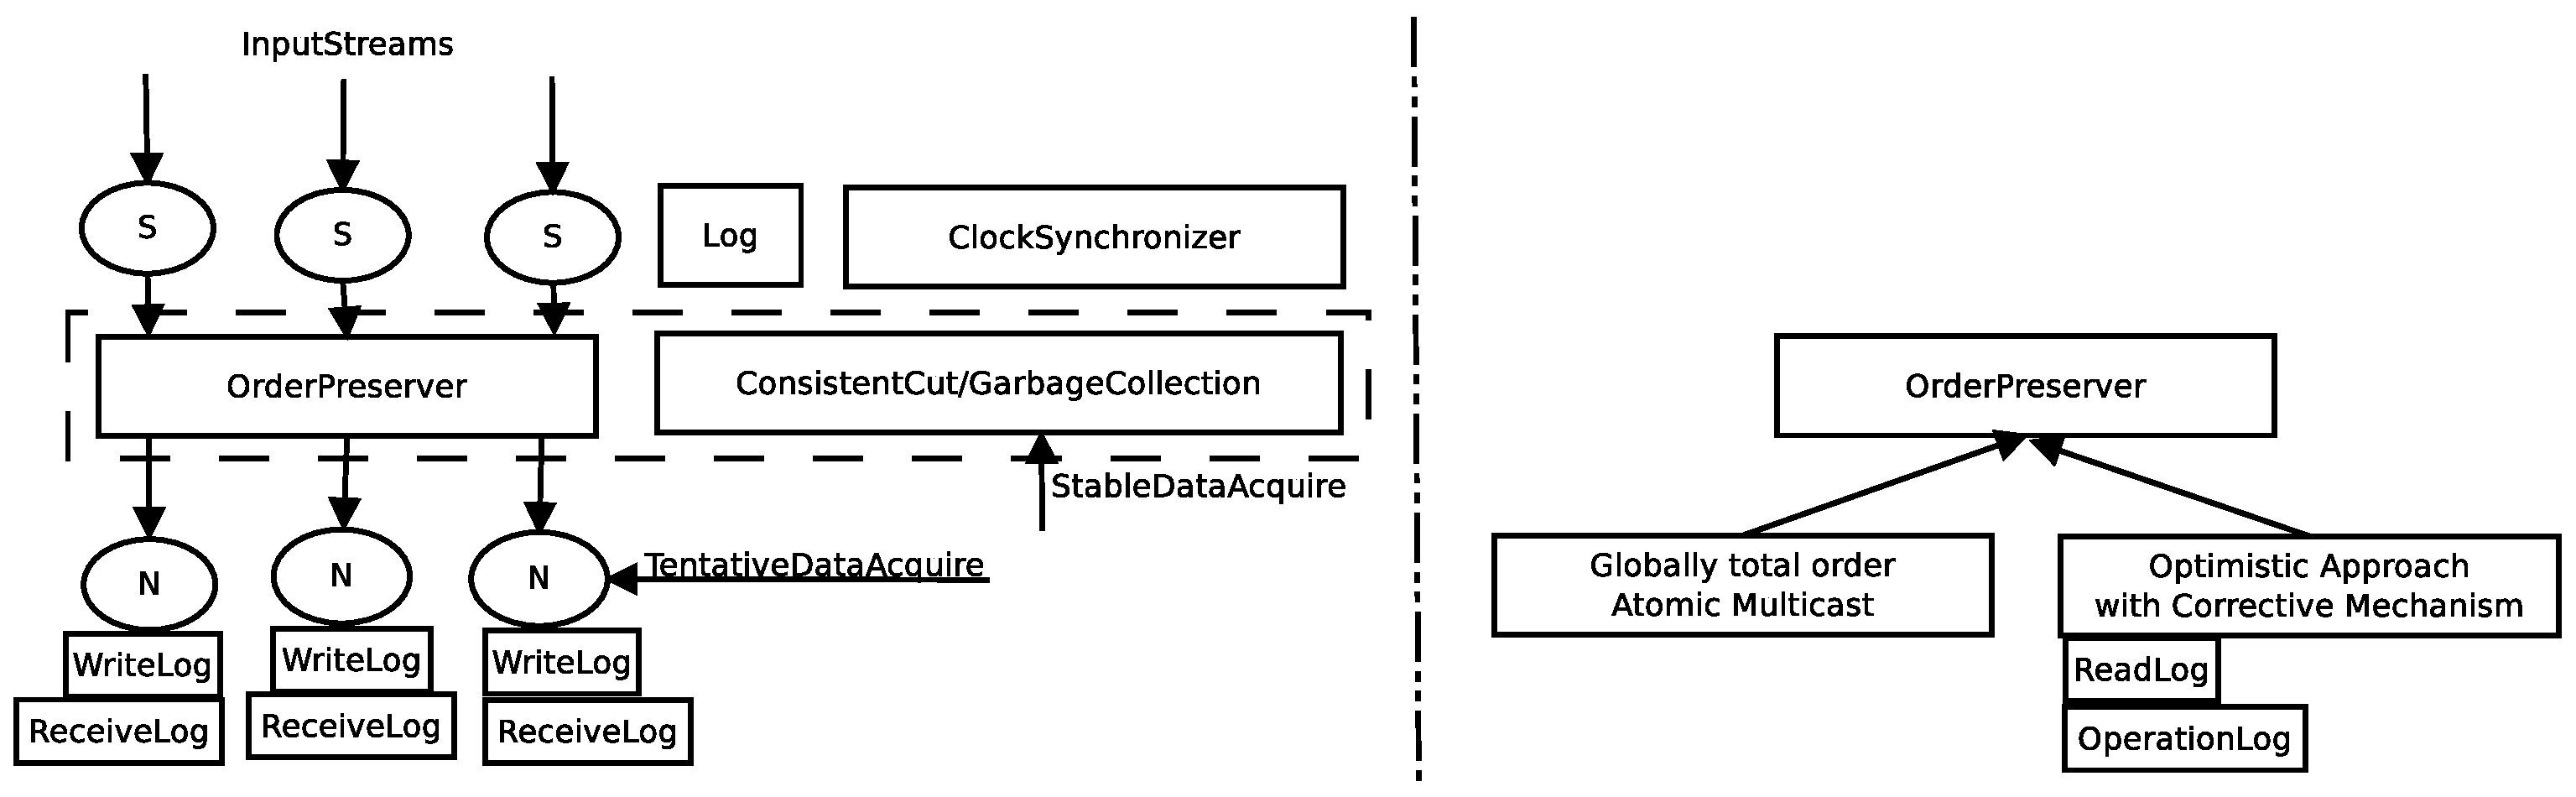
\includegraphics[width=7in]{dynamicArchitecture.eps}
\vspace{-3mm}
\caption{Run-time system architecture. The only part which is application (language) dependent is in the dashed rectangle. On the right, two possible types for the OrderPreserver component is shown.}
\label{fig:dynamicArchitecture}
\vspace{-2mm}
\end{figure*}
The global design of our system is shown in Figure~\ref{fig:dynamicArchitecture}. In a case of using language different than M3, only the components in the dashed rectangular in Figure~\ref{fig:dynamicArchitecture} need to be changed. (For example, we may even need to take care about W-W dependency violation, if the language supports other operations between lhs and rhs beside +=.) Here, the OrderPreserver will be explained in details; more details about other components can be found in SemesterPaper.pdf.

\textbf{The OrderPreserver.} This component is responsible for preserving a unique causal shuffle in the system. A traditional solution is to use atomic multicast for a trigger instantiation spreading. We will describe this approach in detail, and then explain why our Optimistic approach is much better.

Groups of nodes that are informed about a trigger TS from a switch may overlap on some destinations with one another. In the context of atomic multicast, we previously introduced local and total global order. We will show that local total order is not enough for atomicity guarantee.

\begin{example} \em
\label{ex:transitiveCyclic}
Let's take a look at the following trigger and its instantiation:
\begin{verbatim}
ON +R(A, B){
   m1[B]+=m1[A];
}
TS1: R(1,2)
TS2: R(2,3)
TS3: R(1,3)
\end{verbatim}
\end{example}
We assume that these trigger instantiations may arrive from different switches, and each map is stored on separate node. A possible trigger TS arrival on different nodes are shown in Figure~\ref{fig:transitiveCyclic}. Although all the triggers appear in the same order on all the overlapping destinations (conditions for local total order), the atomicity is broken, since TS3 cannot at the same time appear before TS1 and after TS2. Global total order disallows such transitive cyclic executions. Due to data dependencies among map computations, it is necessary to preserve global total order.
\begin{figure}[!t]
\centering
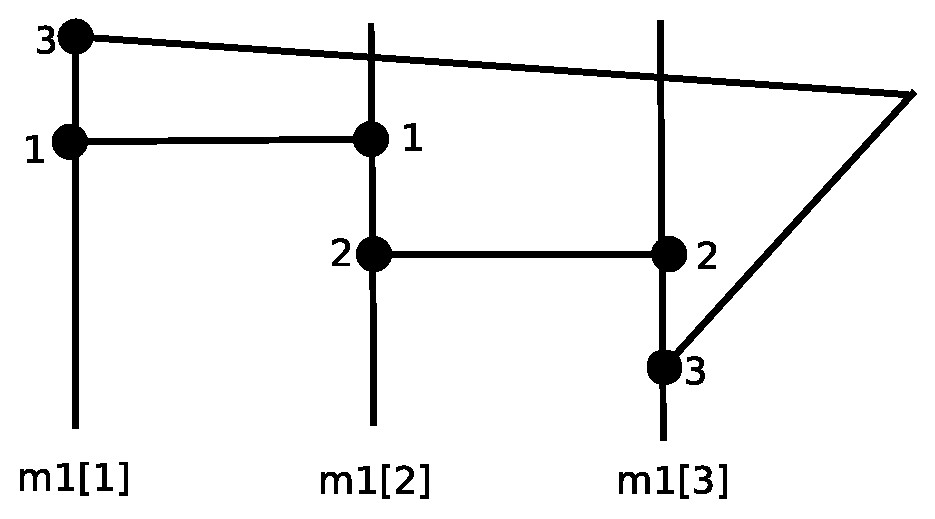
\includegraphics[width=3in]{transitiveCyclic.eps}
\vspace{-3mm}
\caption{Vertical lines represents maps, while horizontal connections represents trigger timestamps affecting different maps. Each map is stored on a separate node.}
\label{fig:transitiveCyclic}
\vspace{-2mm}
\end{figure}

It is also very interesting that the author in~\cite{Birman06} in chapter 17.3 claims that he ''has never encountered a real-world application in which global total order is needed``.

Although the overhead for preserving global total order in atomic multicast is high when there is many overlapping destinations, situations in Example~\ref{ex:transitiveCyclic} are not expected to appear very frequently. 

\begin{example} \em
\label{ex:allowedCyclic}
In a case when trigger instantiations issued at the approximately same time are not causally ordered, total order on nodes may differ from each other, as long as it still provides a unique causal shuffle. In this example, even local total order is too restrictive:
\begin{verbatim}
ON +R(A){
   m1[A]+=m0;
}
TS1: R(1)
TS2: R(2)
\end{verbatim}
\end{example}
If on the node containing m1[1] arrives trigger TSs in order TS1, TS2, and on the node containing m1[2] arrives TS2, TS1, the final result will be the same, since m1[1] and m1[2] are not causally ordered.

Now we will compare the Optimistic approach versus the multicast primitive:
\begin{enumerate}[(1)]
 \item Using multicast primitive guarantee correct execution with less machinery, no ReadLog and OperationLog required anymore. Furthermore, corrective updates (including recursive ones) never occur.
 \item When multicast primitive is used, there is no possibility for trigger instantiation cycles. By avoiding dependency cycles, there is no way to violate causal relations. The Optimistic approach introduces a global total order before even before processing trigger instantiations, but apply corrective updates only if causal relations are broken within this global order.
 \item In the Optimistic approach, due to different speed/load on different switches/nodes, it is entirely possible that some triggers occurred at distant point in time, thus not violating atomicity, need to be reordered by executing corrective updates. 
 \item A huge disadvantage of the multicast primitive is high overhead. However, it is to be hoped that latency will be constant during execution if destinations' overlapping is not very frequent.
\end{enumerate}

\section{Possible directions for research}
\vspace{2mm}

\textbf{The paper structure improvement.} The global organization of the paper will be as follows. First, roles (Source, Computation and Destination Nodes) will be presented in contrast with Dynamo~\cite{decandia07} where there is no dependencies among keys updated. Second, in context of multiple input points in systems necessity of corrective updates will be explained. The need for ``apologies`` or corrective actions is mentioned in~\cite{alvaro11}. In contrast to Bayou~\cite{petersen97}, re-execution in case of corrective updates implies only those maps that are causally ordered with a changed one.

\textbf{The OrderPreserver implementation.}
Most of the group communication tools stress on reliability, which is not a priority for us right now, and infer high latency. An alternative is to implement our primitive from scratch taking into account causal (R/W) relations of a particular language.
 
{
\bibliographystyle{ieeetr}
\bibliography{refs,main,candRefs}
}

\newpage

\end{document}